% !TEX TS-program = pdflatex
% !TEX encoding = UTF-8 Unicode

% This is a simple template for a LaTeX document using the "article" class.
% See "book", "report", "letter" for other types of document.

\documentclass[11pt]{article} % use larger type; default would be 10pt

\usepackage[utf8]{inputenc} % set input encoding (not needed with XeLaTeX)

%%% Examples of Article customizations
% These packages are optional, depending whether you want the features they provide.
% See the LaTeX Companion or other references for full information.

%%% PAGE DIMENSIONS
\usepackage{geometry} % to change the page dimensions
\geometry{a4paper} % or letterpaper (US) or a5paper or....
% \geometry{margin=2in} % for example, change the margins to 2 inches all round
% \geometry{landscape} % set up the page for landscape
%   read geometry.pdf for detailed page layout information

\usepackage{graphicx} % support the \includegraphics command and options

% \usepackage[parfill]{parskip} % Activate to begin paragraphs with an empty line rather than an indent

%%% PACKAGES
\usepackage{booktabs} % for much better looking tables
\usepackage{array} % for better arrays (eg matrices) in maths
\usepackage{paralist} % very flexible & customisable lists (eg. enumerate/itemize, etc.)
\usepackage{verbatim} % adds environment for commenting out blocks of text & for better verbatim
\usepackage{subfig} % make it possible to include more than one captioned figure/table in a single float
% These packages are all incorporated in the memoir class to one degree or another...

\usepackage{hyperref}
\usepackage{amsmath, amssymb}
\usepackage{bbm}
%%% HEADERS & FOOTERS
\usepackage{fancyhdr} % This should be set AFTER setting up the page geometry
\pagestyle{fancy} % options: empty , plain , fancy
\renewcommand{\headrulewidth}{0pt} % customise the layout...
\lhead{}\chead{}\rhead{}
\lfoot{}\cfoot{\thepage}\rfoot{}

%%% SECTION TITLE APPEARANCE
\usepackage{sectsty}
\allsectionsfont{\sffamily\mdseries\upshape} % (See the fntguide.pdf for font help)
% (This matches ConTeXt defaults)

%%% ToC (table of contents) APPEARANCE
\usepackage[nottoc,notlof,notlot]{tocbibind} % Put the bibliography in the ToC
\usepackage[titles,subfigure]{tocloft} % Alter the style of the Table of Contents
\renewcommand{\cftsecfont}{\rmfamily\mdseries\upshape}
\renewcommand{\cftsecpagefont}{\rmfamily\mdseries\upshape} % No bold!

%%% END Article customizations

%%% The "real" document content comes below...

\title{Note scattering transform et wavelet leaders}
\author{Leo Davy}
%\date{} % Activate to display a given date or no date (if empty),
         % otherwise the current date is printed 

\begin{document}
\maketitle

\section{Scattering transform}
\par
Soit $G$ un groupe de rotations $r$ d'angles $\frac{2k\pi}{K}$, on note les ondelettes obtenues à partir d'un filtre passe bande $\psi$ \footnote{Dans les références, l'ondelette (complexe) de Morlet est toujours utilisée ("afin d'avoir un ensemble parcimonieux de coefficients non négligeables")}:
\begin{equation}
	\psi_\lambda(u) = 2^{-2j}\psi (2^{-j}r^{-1}u),\quad \text{avec $\lambda=2^{-j}r$.}
\end{equation}
Ainsi, si $\hat{\psi}$ est centré à la fréquence $\eta$, alors $\hat{\psi}_{2^{-j}r}$ est centré en $2^{-j}r\eta$, avec un support de taille proportionnelle à $2^{-j}$ (donc en augmentant $j$ on analyse à une fréquence plus basse et de façon plus locale (dans le domaine de Fourier)). 
\newline

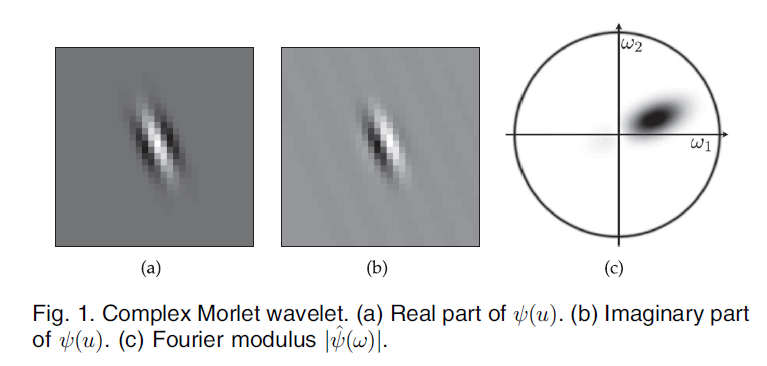
\includegraphics[width=\textwidth]{wav_morlet}

\par
A l'ordre 1, les coefficients de scattering d'un signal $x$ sont définis par 
\begin{equation}
	Sx(u,\lambda,\alpha) = \rho(x\star \psi_{\lambda,\alpha})\star \phi_J(2^Ju)
\end{equation}
où $\psi_{\lambda,\alpha} = Re(e^{-i\alpha}\psi_{\lambda})$, et $\rho$ est un ReLU, $x\mapsto x_+$. L'action du ReLU permet de récupérer seulement les coefficients d'ondelettes positivement corrélés\footnote{Plus précisément, ayant une partie réelle positive après déphasage d'angle $\alpha$, mais par la suite on oublie $\alpha$ et on utilise directement le module complexe.} avec le signal. La convolution par $\phi_J$, une gaussienne permet d'éliminer les variations locales (à une échelle plus fine que $2^J$).
\par
L'information perdue en moyennant avec $\phi_J$ est récupérée par les coefficients d'ordre 2, en appliquant à $\rho(x\star\psi_{\lambda,\alpha})$ une transformée en ondelette, puis on réeffectue un moyennage avec $\phi_J$:
\begin{equation}
	Sx(u,\lambda_1, \lambda_2,\alpha_1,\alpha_2) = \rho(\rho(x\star\psi_{\lambda_1, \alpha})\star\psi_{\lambda_2, \alpha_2})\star\phi_J(2^Ju).
\end{equation}
Afin de réduire le nombre de coefficients, le ReLU qui dépend de la phase est remplacé par un module complexe, ce qui donne les coefficients de second ordre:
\begin{equation}
	Sx(u,\lambda_1, \lambda_2) = ||x\star\psi_{\lambda_1}|\star \psi_{\lambda_2}|\star \phi_J(2^Ju)
\end{equation}
où $|\lambda_2|<|\lambda_1|$ ($j_2>j_1$) (on part des plus hautes fréquences et on récupère les moins hautes fréquences au fur et à mesure).
\newline
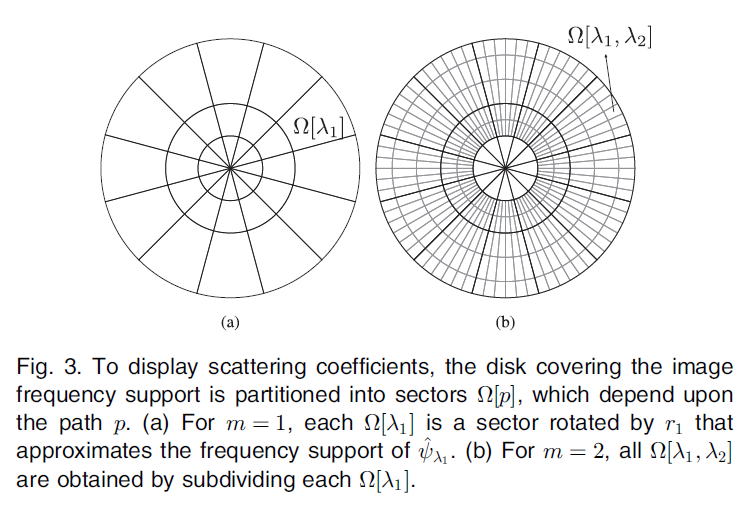
\includegraphics[width=\textwidth]{scat_coef}
Pour généraliser les notations à des ordres plus grands, on peut noter $p=(\lambda_1, \cdots, \lambda_m)$ un chemin, et définir
\begin{equation}
	U[p](x) = |\cdots||x\star\psi_{\lambda_1}|\star\psi_{\lambda_2}|\cdots|\star\psi_{\lambda_m}|
\end{equation}
et $U[\emptyset]x = x$,
et on a les coefficients de scattering en $u$ au bout du chemin $p$
\begin{equation}
	S[p]x(u) = U[p]x\star\phi_{2^J}(u).
\end{equation}
\newline

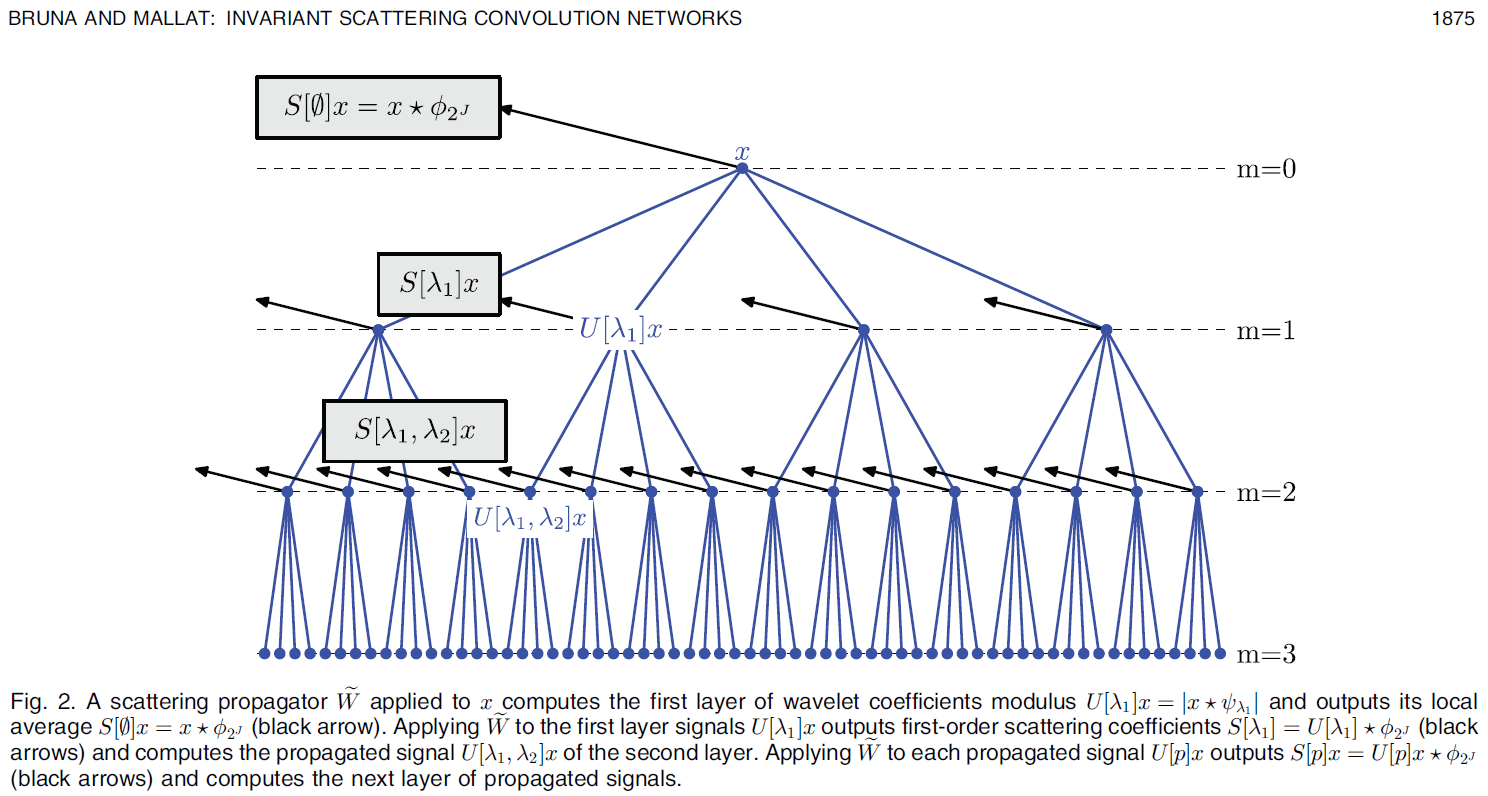
\includegraphics[width=\textwidth]{scat_net}

\par
Quelques propriétés :
\begin{enumerate}
	\item Invariance par translation (grâce à $\star\phi_J$ (?))
	\item Possible d'adapter à d'autres symétries (rotation, changement d'échelle, ...)
	\item En notant $Sx =\{S[p]x\}_{p\in\mathcal{P}_\infty}$:
		\begin{equation}
			||Sx||_2^2 = \sum_{p\in\mathcal{P}_\infty}||S[p]x||^2
		\end{equation}
	\item Lipschitz continue par rapport aux déformations, soit $x_\tau(u) = x(u-\tau(u))$, alors
	\begin{equation}
		||Sx_\tau - Sx||\leq C|\bar m|||x||(2^{-J}||\tau||_\infty + ||\nabla \tau||_\infty)
	\end{equation}
	\item $S$ est non-expansive (car la transformée en ondelette $W$ et le module sont non-expansifs)
	\item Conservation de l'énergie si $W$ est unitaire\footnote{$\mathcal{P}^m$ est l'ensemble des chemins de longueur $p$.}
	\begin{equation}
		||x||^2 = \sum_{m=0}^{l}\sum_{p\in\mathcal{P}^m}||S[p]x||^2 + \sum_{p\in\mathcal{P}^{l+1}}||U[p]x||^2
	\end{equation}
	\item Réseau peu profond (car le dernier terme de l'équation précédente tend vers 0, donc l'énergie se concentre sur les premières couches)
	\item Nombre total de coefficients, avec profondeur $\bar m$, $K$ rotations,
		\begin{equation}
			P = N2^{-2J}\sum_{m=0}^{\bar m} K^m\binom{J}{m}
		\end{equation} 
	\item Compléxité de calcul de $\bar m$ couches
	\begin{equation}
		\mathcal{O}\left(\left(\frac{K}{3}\right)^{\bar m} N\log{N}\right)
	\end{equation}	
\end{enumerate}
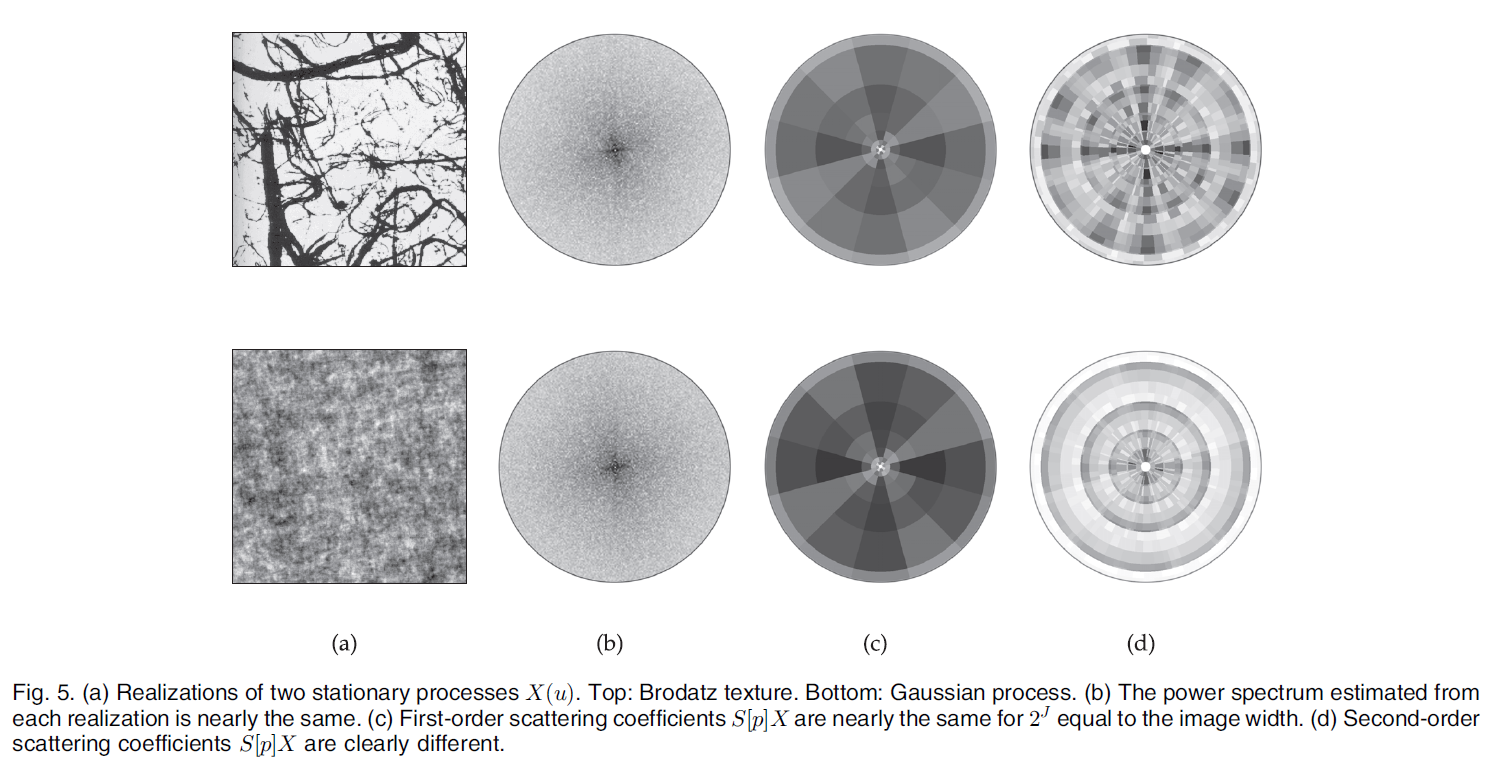
\includegraphics[width=1.2\textwidth]{scat_station}
Quelques applications :
\begin{enumerate}
	\item Processus stationnaires, les coefficients de scattering sont aussi stationaires, la variance est conservée
		\begin{equation}
			\sum_{p\in\mathcal{P}_\infty} \mathbb{E}|S[p]X|^2 = \mathbb{E}|X|^2
		\end{equation}
		et la variance des coefficients d'une ondelette $\psi_\lambda$ est donnée par
		\begin{equation}
			\sum_{p\in\mathcal{P}_\infty }\mathbb{E}|S[\lambda + p]X|^2 = \mathbb{E}|X\star \psi_\lambda|^2.
		\end{equation}
		Peut distinguer des textures qui ont des seconds moments identiques, mais des moments de plus grand ordre distincts.
	\item PCA/classification: Soit $k$ une classe, et $X_k$ des réalisations de la classe $k$, alors les coefficients moyens sont donnés par $\mathbb{E} SX_k$. La différence $SX_k - \mathbb{E}SX_k$ peut être approximée dans un espace de dimension $d$ ($d<<P$ où $P$ est le nombre total de coefficients), et la meilleure approximation est donnée par les $d$ principaux vecteurs de la matrice de covariance de $SX_k$, on note $V_k$ l'espace linéaire engendré par les $d$ vecteurs principaux. Cela nous donne un espace affine pour chaque classe $k$
		\begin{equation}
			\mathbb{A}_k = \mathbb{E}SX_k + V_k
		\end{equation}
		et on associe à un nouveau signal $x$ sa classe :
		\begin{equation}
			\hat{k}(x) = argmin_{k\leq C}||Sx - P_{\mathbb{A}_k}(Sx)||
		\end{equation}
	\item Classification : On apprend un classifieur (PCA ou SVM) à partir des coefficients de scattering (qui par invariance, ne dépendent pas de la position, rotation, éclairage, ...), état de l'art sur MNIST, USPostalService et CUReT (classification de texture)
\end{enumerate}
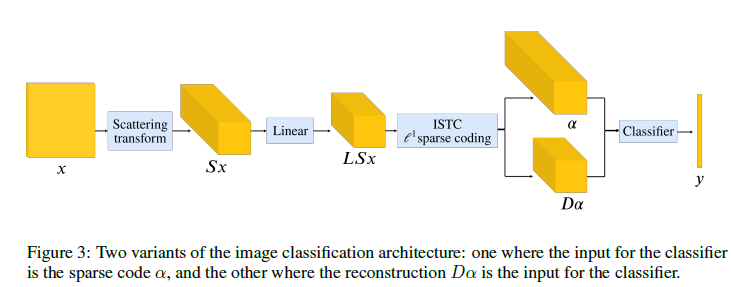
\includegraphics[width=\textwidth]{scat_clas}
Quelques références :
\begin{enumerate}
	\item  Référence principale \emph{Invariant Scattering Convolution Networks}, \textsc{Bruna, Mallat} \url{http://people.ee.duke.edu/~lcarin/Bruna_Mallat.pdf}
	\item Détails pour de la classification et liens avec opérateurs proximaux et (A)(L)ISTA \emph{Deep Network classification by scattering and homotopy dictionary learning}, \textsc{Zarka, Thiry, Angles, Mallat}, \url{https://arxiv.org/abs/1910.03561}
	\item Détails sur comment construire des coefficients de scattering ayant des groupes d'invariance prédéfinis, \emph{Group invariant scattering}, \textsc{Mallat}, \url{https://www.di.ens.fr/~mallat/College/CPAM-Mallat-Scat.pdf}
\end{enumerate}

\section{Wavelet leaders}
	Quelques définitions, pour $x$ un signal, $a$ l'echelle, $k$ position et $T_x(a,k)$ une quantité multi-échelle :
	\begin{enumerate}
		\item Fonction de structure :
			\begin{equation}
				S(a,q) = \frac{1}{n_a}\sum_{k=1}^{n_a} |T_x(a,k)|^q = \mathbb{E}_{k\in\lambda_a} |T_x(a,k)|^q \sim a^{\zeta(q)}
			\end{equation}
			correspond au $q$-ème moment de $T_x(a,\cdot)$ (donc un moment généralisé de $x$ à l'échelle $a$) en donnant le même poids à tous les $n_a$ coefficients accessibles à l'échelle $a$ (donc invariant par tranlation). 
		\item Fonction d'échelle $\zeta(q)$ donne le taux de croissance de $S(a,q)$ (en fonction de $a$).
		\item Régularité en $u$ :
			\begin{equation}
				h(u) = \liminf_{a\to 0} \frac{\log(T_x(a, k(u))}{log(a)}
			\end{equation}
			donne la régularité (minimale) du signal en $u$ aux échelles les plus fines.\footnote{Si $h$ ne dépend pas de $u$, alors $h = \zeta(1)$ (?)} 
	\end{enumerate}
	Et en adaptant les définitions précédentes aux coefficients d'ondelettes
	\begin{align}
		c_{j,k}^{(i)} 	&= \int_{\mathbb{R}^d} X(u)2^{-dj}\psi^{(i)}(2^{-j}u -k) \,du\\
					&= \langle X, \psi_{j,k}^{(i)} \rangle = X\star \psi_{j}^{(i)}(k)
	\end{align}
	et pour alléger les notations, on peut poser
	\begin{equation}
		c_{\lambda}^p := \sum_i |c_{\lambda}^{(i)}|^p,\quad\text{où $\lambda=(j,k) $},
	\end{equation}
	 et on a alors:
	\begin{enumerate}
		\item Fonction de structure :
			\begin{equation}
				S(j,p) = 2^{dj}\sum_k\sum_i |c_{j,k}^{(i)}|^p = 2^{dj}\sum_k c_{j,k}^p
			\end{equation}
		\item Fonction d'échelle :
			\begin{equation}
				\eta(p) = \liminf_{j\to-\infty} \frac{\log(S(j,q))}{\log(2^j)}
			\end{equation}
		\item Leaders :
			\begin{equation}
				l^p(j,k) = \left( \sum_{j'\leq j, \lambda'\subset 3\lambda} 2^{-d(j-j')} c_{\lambda'}^p \right)^{\frac{1}{p}}
			\end{equation}
		\item $p$-exposant :
			\begin{equation}
				h_p(u) = \liminf_{j\to -\infty} \frac{\log(l_{\lambda_j(u)}^{(p)})}{\log(2^j)}
			\end{equation}
	\end{enumerate}

	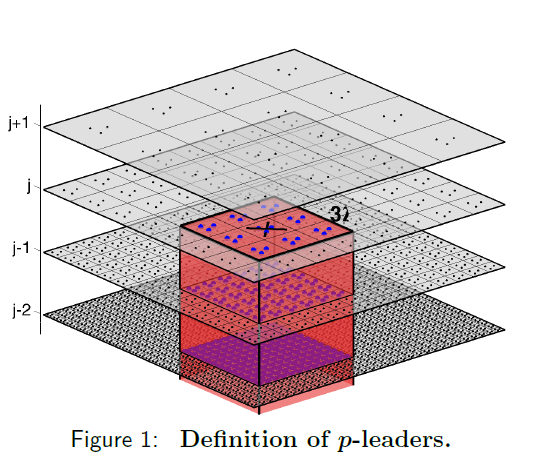
\includegraphics[width=0.8\textwidth]{p_lead}
	\subsection{Leaders et coefficients de scattering}
	Le cas $p=\infty$ des leaders correspond à la définition classique des wavelets leaders :
	\begin{equation}
		l_\lambda^{p=\infty} = \sup_{\lambda'\subset 3\lambda}|c_{\lambda'}^{(i)}| = \sup_{\lambda'} |c_{\lambda'}|.
	\end{equation}
	Le cas $p=1$ semble correspondre à la norme 1 des coefficients de scattering à une couche avec des fréquences arbitrairement grandes :
	\begin{align}
		l_\lambda^{p=1} 	&:= \sum_{j'\leq j, \lambda' \subset 3\lambda} \sum_i |c_{\lambda'}^{(i)}| 2^{-d(j-j')} \\
						&= 2^{-dj}\sum_i \sum_{j' \leq j} \sum_{\lambda_{j'} \subset 3\lambda} \sum_{k\in \lambda_{j'}} |c_{j',k}^{(i)}| 2^{dj'} \\
						&= 2^{-dj}\sum_i \sum_{j' \leq j} \sum_{\lambda_{j'} \subset 3\lambda} \sum_{k\in \lambda_{j'}} |X\star\psi_{j'}^{(i)}| (k) \\
						&= 2^{-dj}\sum_i \sum_{j' \leq j} \sum_{\lambda_{j'} \subset 3\lambda} \sum_{k\in \mathbb{Z}^d} |X\star\psi_{j'}^{(i)}| (k) \mathbbm{1}_{3\lambda}(k)\\
						&= 2^{-dj}\sum_i \sum_{j' \leq j} \sum_{k\in \mathbb{Z}^d} |X\star\psi_{j'}^{(i)}| (k) \mathbbm{1}_{3\lambda}(k)\\
						&= 2^{-dj}\sum_i \sum_{j' \leq j} \sum_{k\in \mathbb{Z}^d} |X\star\psi_{j'}^{(i)}| \star \mathbbm{1}_{[-2^{j'}, 2^{j'}]^d}(2^j k)\\
						&= 2^{-dj}\sum_i \sum_{j' \leq j} \sum_{k\in \mathbb{Z}^d} S^{(i)}[j']x(k)\\
	\end{align}
	où $S^{(i)}[j']x(k)$ correspondent à des coefficients de scattering pour lesquels on a remplacé la convolution par une gaussienne $\phi_J$ par la convolution avec une indicatrice sur un cube dyadique.

\end{document}
